\documentclass[12pt]{scrbook}
\usepackage{graphicx} % Required for inserting images
\usepackage{amsmath}        %mathematische Symbole
\usepackage[ngerman]{babel}  %Latex kann dann deutsch
\usepackage{graphicx}       %zum Einbinden der Bilder
\usepackage{wrapfig}        
\usepackage{latexsym}       
\usepackage{tabularx}       %für Tabellen, welche sich dynamisch der Textbreite anpassen
\usepackage{lmodern}        %Schrift wird in PDFs flüssiger
\usepackage{pdfpages}       %für Einbinden von PDF-Seiten in Fehlerversuch GeoMat
\usepackage{footnote}       %Ermöglicht Fußnoten in gleitenden Umgebungen
\usepackage{caption}        
\usepackage{enumitem}       %für nicht-einrücken in Lernzielen (Bio-Anleitungen)
%\usepackage{layout}         %für Debugging: \layout nutzen!
\usepackage{float}          %Juli 2019 eingefügt
\floatplacement{figure}{H}  %Definition der default-Platzierung: H, bedeutet /genau wirklich hier/
\usepackage{longtable}      %kann unter anderem Zeilenumbrüche in Tabellen
\usepackage{color}					%zum definieren von eigenen Farben dh. definecolor-Befehl für lightgray
\usepackage{colortbl}       %damit Farben auch in Tabellen funktionieren
\usepackage{units}          %damit man Einheiten korrekt darstellen kann: \unit[]{}
\usepackage{hyperref}
\usepackage{microtype}      %somit weniger overful-Box-Meldungen, bessere Umbrüche am Zeilenende
\usepackage{libertine}     %wesentlich schönere Schriftart!

\parindent0pt

\newcommand\einfachleer{\\[5mm]
\underline{\hspace{\linewidth}} \\[5mm]}

\newcommand\doppeltleer{\\[5mm]
\underline{\hspace{\linewidth}}\\[5mm]
\underline{\hspace{\linewidth}}\\[5mm]}

\newcommand\dreifachleer{\\[5mm]
\underline{\hspace{\linewidth}}\\[5mm]
\underline{\hspace{\linewidth}}\\[5mm]
\underline{\hspace{\linewidth}}\\[5mm]}

\newcommand{\hdick}{\noalign{\hrule height1.4pt}}
\newcommand{\beq}{\begin{equation}}
\newcommand{\eeq}{\end{equation}}
\newcommand{\gl}[1]{Gl.~(\ref{#1})}
\newcommand{\abb}[1]{Abb.~\ref{#1}}

\newcommand{\D}{\displaystyle}
\newcommand{\be}{\begin{eqnarray}}
\newcommand{\ee}{\end{eqnarray}}
\newcommand{\beo}{\begin{eqnarray*}}
\newcommand{\eeo}{\end{eqnarray*}}
\newcommand{\ale}{\mbox{\ \raisebox{-1ex}{$\stackrel{\textstyle<}{\sim}$}\ }}
\newcommand{\age}{\mbox{\ \raisebox{-1ex}{$\stackrel{\textstyle>}{\sim}$}\ }}
\newcommand{\chem}[2]{\mathrm{#1}_{#2}}
\newcommand{\MR}{\mathrm}

\newcommand{\rb}[1]{\raisebox{-1.5ex}[1.5ex]{#1}}

\newcommand{\element}[3]{\makebox[0cm][r]{$^{#3}$}\makebox[0cm][r]{$_{#2}$}#1} %für chemische Elemente: \element{U}{92}{238}

\setlength{\textheight}{26.0cm}
\setlength{\topmargin}{-2.2cm}
\setlength{\footskip}{1cm}
\setlength{\oddsidemargin}{0.0cm}
\setlength{\evensidemargin}{0.0cm}
\setlength{\hoffset}{-1.5cm}
\setlength{\textwidth}{19cm}

%Achtung: Breiten Minipage und parbox unterschiedlich definiert!
\newcommand\minipagewidth{18.8cm} % = textwidth - 0.2cm
\newcommand\parboxwidth{18.6cm}   % = textwidth - 0.4cm

\title{Python Versuch Test File}
\author{maximilian.kuehlkamp }
\date{July 2023}

\begin{document}

\chapter{Datenauswertung mit Python (PYT)}

\textbf{Wichtige Hinweise:} 
\begin{itemize}
    \item Bringen Sie bitte einen Laptop mit der installierten Software (siehe \autoref{PY:Vorbereitung}), eine Maus und ein Netzteil mit. Melden Sie sich bitte \textbf{rechtzeitig} bei Ihrer Versuchsbetreuerin oder Ihrem Versuchsbetreuer, falls Sie keinen Laptop zum Versuch mitbringen können oder falls Probleme bei der Installation der Software auftreten.
    \item Die sinnvolle Teilnahme am Versuchstag erfordert eine ausführliche Vorbereitung mit dem Einführungs-Notebook (siehe Abschnitt \ref{PY:Vorbereitung})
\end{itemize}


\section{Ziel des Versuchs}

In den Naturwissenschaften ist die computergestützte Datenauswertung nicht mehr wegzudenken. In der Schule lernt man in dem Kontext, wenn überhaupt, die digitale Messdatenanalyse mit Hilfe von \textit{Microsoft Excel} kennen. \textit{Excel} bietet zwar eine einfache und grafisch ansprechende Umgebung zur Berechnung und Darstellung von Daten, bei der Arbeit mit großen Datenmengen kommt \textit{Excel} jedoch schnell an seine Grenzen. Es ist somit nicht verwunderlich, dass in der naturwissenschaftlichen Forschung in der Regel \textbf{Programmiersprachen} zur \textbf{Simulation und Analyse} verwendet werden. Die Liste der Programmiersprachen ist lang und jede Sprache hat in verschiedenen Anwendungsbereichen ihr Stärken und Schwächen. In diesem Versuch \textbf{lernen Sie den Umgang}  mit der Programmiersprache \textbf{\textit{Python}}. \textit{Python} enthält viele Pakete mit Funktionen die \textbf{speziell für die Messdatenanalyse und -darstellung} ausgelegt sind und bietet durch eine vereinfachte Syntax einen \textbf{leichten Einstieg} in die Programmierung. Zur Strukturierung der Auswertungsschritte werden \textbf{\textit{Jupyter-Notebooks}} verwendet. Diese wurden explizit zur Datenauswertung entwickelt und bestehen aus sogenannten Code- und Text-Zellen die ein schrittweises Auswerten ermöglichen.\\
Dieser Versuch soll Sie dazu befähigen, \textbf{\textit{Python}} zusammen mit \textit{Jupyter-Notebooks} als \textbf{sinnvolle Alternative} zu \textit{Excel} als \textbf{Auswertungsmedium} zu verwenden.



\section{Versuchsvorbereitung}
\label{PY:Vorbereitung}

Die Vorbereitung auf den Versuch beinhaltet die \textbf{Installation} von \textit{Anaconda} und \textit{Visual Studio Code} sowie die \textbf{Bearbeitung} des \textit{Jupyter-Notebooks} zur Einführung in Python. Das Notebook \textbf{\textit{Einführung\_in\_Python.ipynb}} sowie die dazugehörigen Messdaten \textbf{\textit{Beispiel.csv}} finden Sie im Moodle-Lernraum in dem Ordner \textbf{Versuch-PYT}. Laden Sie direkt den gesamten Ordner herunter. Eine herkömmliche Vorbesprechung entfällt, \textbf{die Installationen und das bearbeitete Notebook werden jedoch zu Beginn des Versuchs von der Versuchsbetreuerin oder dem Versuchsbetreuer kontrolliert}. Eine Teilnahme ohne Vorbereitung ist \textbf{nicht} möglich.




\subsection{Installation}


\subsubsection{Anaconda}
\label{PY:Conda}
Folgen Sie zur Installation folgender Anleitung: \href{https://docs.anaconda.com/free/anaconda/install/windows/}{Anaconda (Windows)}, \href{https://docs.anaconda.com/free/anaconda/install/mac-os/}{Anaconda (macOS)},
\href{https://docs.anaconda.com/free/anaconda/install/linux/}{Anaconda (Linux)}\\
\newline
Überprüfen Sie nach der Installation, ob \textit{Anaconda} richtig installiert wurde, indem Sie den \textit{Anaconda Navigator} öffnen. Falls Sie den Navigator auf Ihrem Laptop nach der Installation nicht finden können, installieren Sie \textit{Anaconda} neu und setzen Sie die Häkchen bei \textit{Add Anaconda3 to my PATH environment variable} und \textit{Add Anaconda to windows startmenu} (nur Windows).


\subsubsection{Visual Studio Code}
Den Download finden Sie hier: \href{https://code.visualstudio.com/download}{Visual Studio Code}.\\
\newline
Einen einfachen Einstieg in die Verwendung von \textit{Visual Studio Code} bietet das folgende deutschsprachige Video: \href{https://www.youtube.com/watch?v=_-IDIkoo2ZA&ab_channel=FabianHiller}{Einführung in Visual Studio Code für Anfänger | 2021}. 
Vor allem die Erklärungen zum Erstellen und Öffnen von Projekten (ab 03:00 min) sowie das Installieren von Erweiterungen (ab 11:26 min) sind hilfreich.\\
\newline
Zur Bearbeitung von \textit{Jupyter-Notebooks} in \textit{Visual Studio Code} benötigen Sie zwei Erweiterungen. Eine Anleitung wie Sie Erweiterungen installieren können finden Sie im oben genannten Video oder hier: \href{https://code.visualstudio.com/docs/editor/extension-marketplace}{Extension Marketplace}.\\
Installieren Sie die Erweiterungen \textbf{\textit{Jupyter}} und \textbf{\textit{Python}}.\\
\newline
Sie sollten nun \textbf{\textit{Anaconda}}, \textbf{\textit{Visual Studio Code}} und die beiden Erweiterungen \textbf{\textit{Jupyter}} und \textbf{\textit{Python}} installiert haben.




\subsection{Bearbeitung des \textit{Jupyter-Notebooks} zur Einführung in Python}

Laden Sie den oben genannten Ordner \textbf{Versuch-PYT} aus dem Moodle-Lernraum herunter. Öffnen Sie nun diesen Ordner im Explorer von \textit{Visual Studio Code} (siehe \href{https://www.youtube.com/watch?v=_-IDIkoo2ZA&ab_channel=FabianHiller}{Einführung in Visual Studio Code für Anfänger | 2021}). Anschließend können Sie über den Explorer das Notebook \textit{Einführung\_in\_Python.ipynb} öffnen. Das Ganze sollte dann in etwa wie in \autoref{explorer} aussehen. 

\begin{figure}[ht]
\center
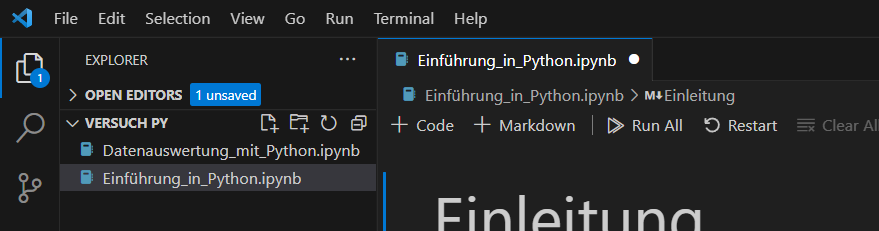
\includegraphics[scale=0.8]{Explorer_VSCode.png}
\caption{Darstellung des Explorers in \textit{Visual Studio Code} nach der Öffnung des Ordners (hier \textit{Versuch PY}) und dem geöffneten Einführungs-Notebook.}
\label{explorer}
\end{figure}

Damit \textit{Python}-Code innerhalb des \textit{Jupyter-Notebooks} ausgeführt werden kann, muss ein Übersetzer ausgewählt werden. Der sogenannte \textit{Interpreter} übersetzt den Code und führt ihn aus. In \textit{Visual Studio Code} wählen Sie den \textit{Interpreter} über die Kommando-Palette aus. Die Kommando-Palette öffnen Sie mit der Tastenkombination STRG+SHIFT+P. In der Suche geben Sie nun \textit{Python: Select Interpreter} ein und wählen es aus. Es öffnet sich anschließend eine Liste mit Ihren \textit{Python}-Installationen (siehe \autoref{selectinterpreter}). Wählen Sie die in \autoref{selectinterpreter} rot markierte Option aus. Bei \textit{macOS} kann der Dateipfad von der Abbildung abweichen. Dort hat der Dateipfad die Form \textit{\textbackslash anaconda3\textbackslash bin\textbackslash python}.

\begin{figure}[ht]
\center
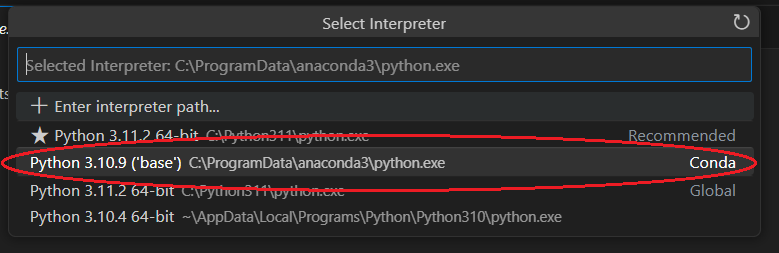
\includegraphics[scale=0.7]{Select Interpreter.png}
\caption{Liste der \textit{Python}-Installationen nach Aufruf von \textit{Python: Select Interpreter} in der Kommando-Palette von \textit{Visual Studio Code}. Die auszuwählende Installation (\textit{Anaconda}) ist rot markiert.}
\label{selectinterpreter}
\end{figure}

Wird in der Liste die \textit{Anaconda}-Installation nicht angezeigt, wurde bei der Installation von \textit{Anaconda} keine Referenz in \textit{Visual Studio Code} hinterlegt. Versuchen Sie zur Behebung des Problems die in Abschnitt ~\ref{PY:Conda} vorgestellte Neuinstallation. Kann das Problem so nicht behoben werden melden Sie sich \textbf{umgehend} bei Ihrer Versuchsbetreuerin oder ihrem Versuchsbetreuer.\\
\newline
Als letzter Schritt, bevor Sie mit der Bearbeitung des Notebooks beginnen können, muss jetzt noch ein Kernel gestartet werden. Der Kernel funktioniert, wie der Name es vermuten lässt, als Prozessor der den \textit{Python}-Code übersetzt. Klicken Sie dafür zuerst rechts oben auf \textit{Select Kernel} (siehe \autoref{selectkernel}) und dann in der geöffneten Auswahl auf \textit{Python Environments...} . Wählen Sie nun in der Liste die bereits im letzten Schritt ausgewählte \textit{Python}-Version (siehe \autoref{auswahlkernel}) aus. Wird anstatt \textit{Select Kernel} nun die \textit{Python}-Version als Kernel angezeigt (siehe rechts in \autoref{auswahlkernel}), ist das Notebook einsatzbereit.\newline 

\textbf{Sie können jetzt mit der Bearbeitung des Einführungs-Notebooks beginn.} 


\begin{figure}[ht]
\center
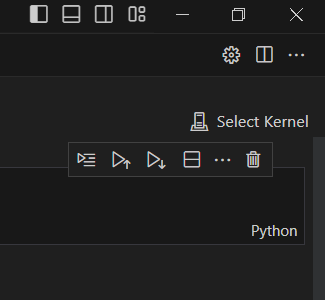
\includegraphics[scale=0.7]{Select_Kernel.png}
\caption{Position der Kernel-Auswahl in \textit{Visual Studio Code}.}
\label{selectkernel}
\end{figure}
\begin{figure}[ht]
\center
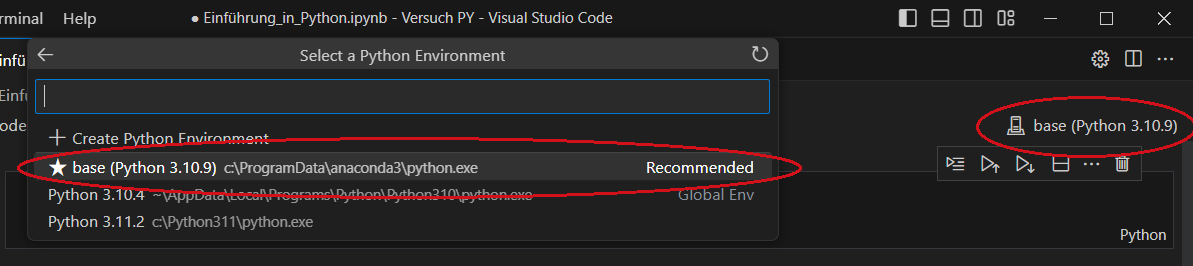
\includegraphics[scale=0.7]{Auswahl_Kernel.png}
\caption{Auswahl der richtigen \textit{Python}-Installation als Kernel.}
\label{auswahlkernel}
\end{figure}



\newpage



\section{Versuchsdurchführung}

Am Versuchstag werten Sie mit Hilfe eines weiteren Notebooks Messdaten des Versuchs zum Federpendel aus. Die Messdaten finden Sie im Moodle-Lernraum. Die physikalischen Grundlagen zum Federpendel können unter folgendem Link nachgelesen werden: \href{https://www.leifiphysik.de/mechanik/mechanische-schwingungen/grundwissen/federpendel}{Federpendel (LEIFIphysik)}.

Laden Sie, falls noch nicht geschehen, den gesamten Ordner \textbf{Versuch-PYT} aus dem Moodle-Lernraum herunter. Dieser beinhaltet neben dem Einführungs-Notebook das Datenauswertungs-Notebook \textbf{\textit{Datenauswertung\_mit\_Python.ipynb}}, den Ordner mit den Messdaten und ein Python-Skript für Hilfestellungen \textbf{\textit{Hilfestellungen.py}}. Nachdem Sie diesen Ordner in dem Explorer von Visual Studio Code geöffnet haben, können Sie mit der Bearbeitung des Datenauswertungs-Notebooks \textit{Datenauswertung\_mit\_Python.ipynb} beginnen. \newline

\textbf{Zusatz:}

Der Versuch wird am Versuchstag nicht von Ihnen selbst durchgeführt. Falls Sie jedoch gerne Zuhause eigene Messdaten aufnehmen möchten, folgt nun die Beschreibung des Versuchs zum Federpendel:

\subsection{Versuch Federpendel}

Um bei der Auswertung die Federkonstante \textit{D} einer Stahlfeder bestimmen zu können, wird mit der App \textit{phyphox} der Beschleunigungsverlauf eines Federpendels bei verschiedenen Massen bestimmt.

\subsubsection{Materialien}
\begin{itemize}
    \item Smartphone mit \textit{phyphox}
    \item Rechteckige Plastiktüte
    \item Stahlfeder
    \item Schlüsselring 
    \item 5 Massenstücke (jeweils 10 bis 30 g)
    \item Kleiderständer (oder andere Befestigungsmöglichkeit)
    \item Waage
\end{itemize}

Ein Experimentierset mit Stahlfeder und Plastiktüte kann nach Absprache mit der Betreuerin bzw. dem Betreuer abgeholt werden.

\subsubsection{Messung mit \textit{phyphox}}

Mit \textit{phyphox} soll der \textbf{Verlauf der Beschleunigung in Bewegungsrichtung} gemessen werden.  Wählen sie hierfür das Experiment \textbf{\textit{Beschleunigung (ohne g)}} aus. Stellen Sie jetzt die Zeitautomatik ein, damit die Messung während der Schwingbewegung startet und keine menschlichen Einflüsse die Bewegung am Start und am Ende beeinflussen. Die Zeitautomatik finden Sie in dem Menü, welches Sie über die drei Punkte rechts oben in der Ecke öffnen können (siehe \autoref{zeitautomatikphyphox}). Geben Sie als Startverzögerung 2 Sekunden und als Dauer des Experiments 10 Sekunden an. Aktivieren Sie die Zeitautomatik. Nach Start der Messung haben Sie jetzt 2 Sekunden Zeit die Feder auszulenken und in Bewegung zu versetzen. Anschließend misst \textit{phyphox} 10 Sekunden lang die Beschleunigung in x-,y- und z-Richtung. Welche Beschleunigungsrichtung für die Messung relevant ist, können Sie im Vorfeld über eine Testmessung herausfinden.

\begin{figure}[ht]
    \center
    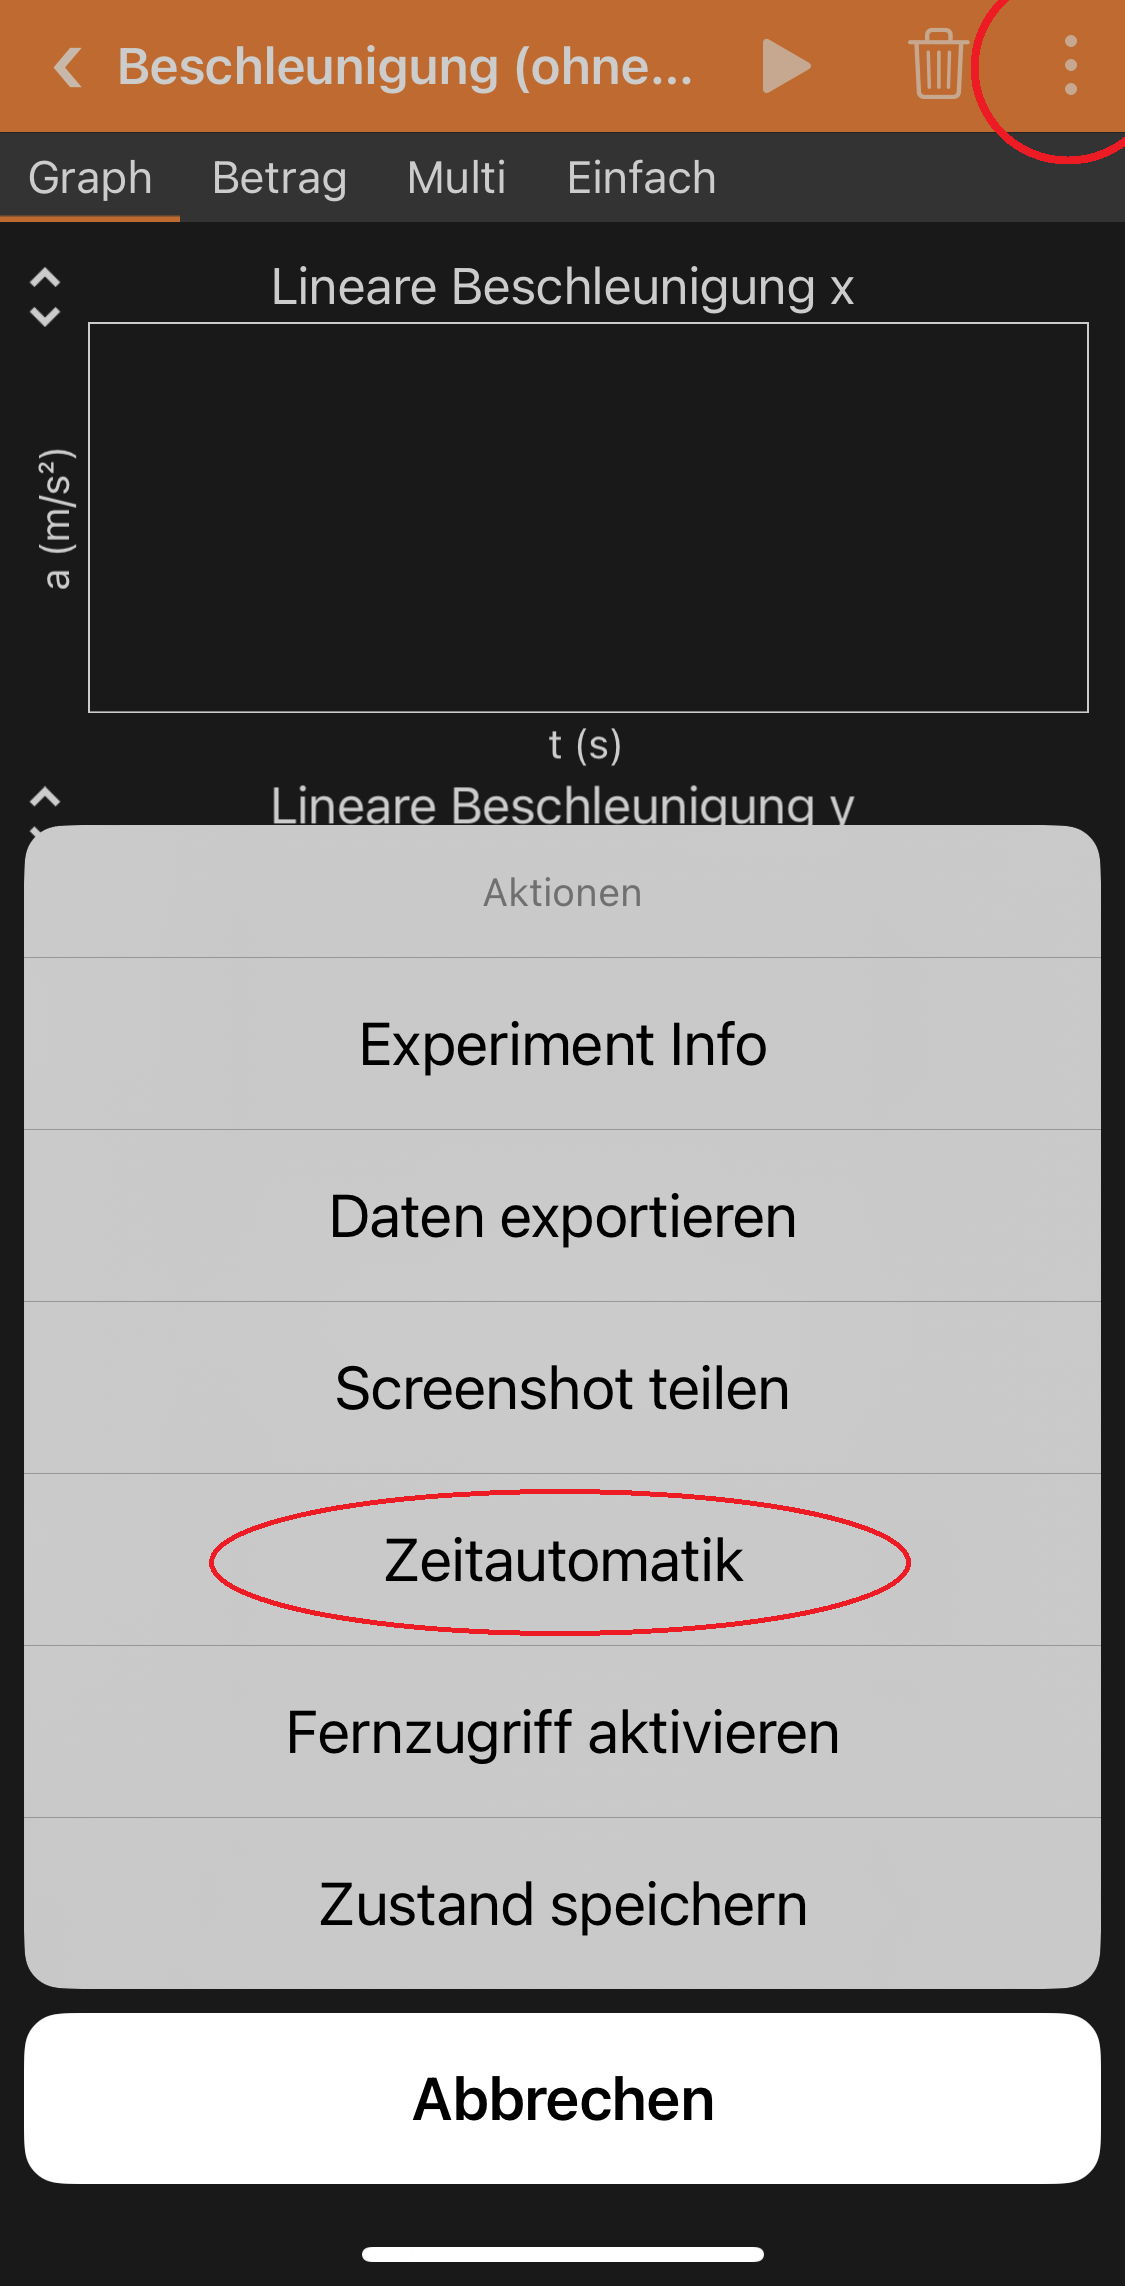
\includegraphics[scale=0.2]{Zeitautomatik.png}
    \caption{Menü innerhalb eines \textit{phyphox}-Experiments. Die drei Punkte zum Öffnen des Menüs und die Auswahl \textit{Zeitautomatik} sind rot hervorgehoben.}
    \label{zeitautomatikphyphox}
\end{figure}


Nach \textbf{jeder Messung} sollten Sie die Messung \textbf{abspeichern}. Öffnen Sie dafür wieder das Menü über die drei Punkte. Wählen Sie jetzt die Option \textit{Daten exportieren} aus. Geben Sie als Datei-Format \textit{CSV (Comma, decimal point)} an und speichern es so ab, dass Sie später mit ihrem Laptop auf die Datei zugreifen können.

\subsubsection{Aufbau}
Befestigen Sie die Stahlfeder mit dem Schlüsselring an einem Haken des Kleiderständers. Legen Sie das Smartphone mit vorbereiteter Messung in die Plastiktüte. Anschließend hängen Sie die Tüte samt Smartphone an die Stahlfeder (siehe \autoref{federaufbau}). Legen Sie die verschiedenen Massen für die jeweilige Messung vorsichtig neben das Smartphone in die Plastiktüte.

\begin{figure}[h]
\center
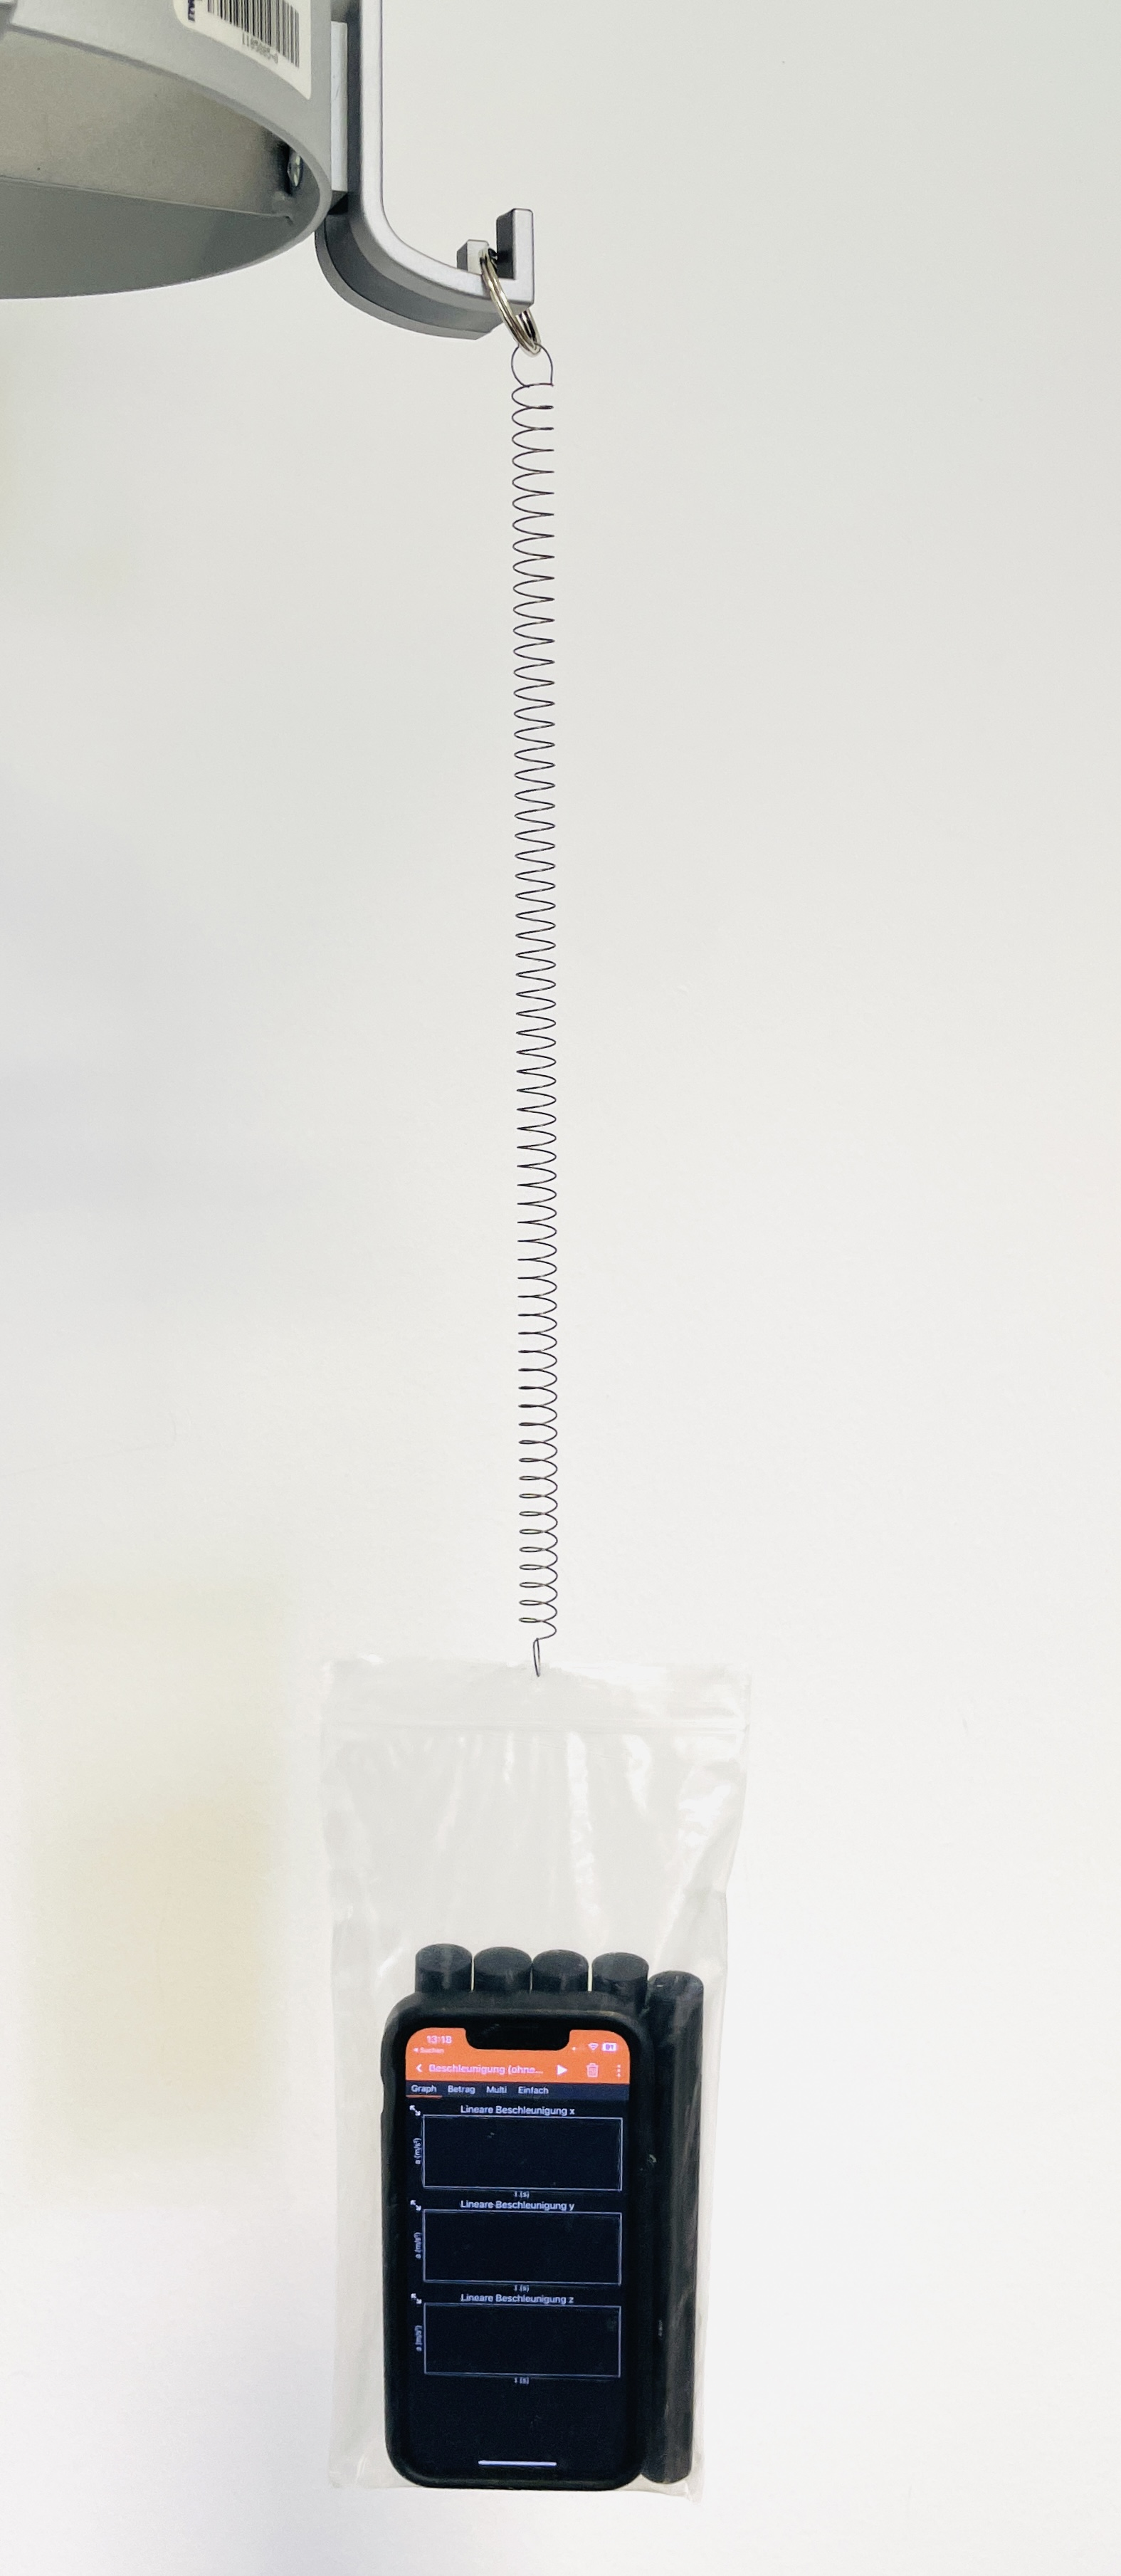
\includegraphics[scale=0.4]{Federpendel.jpg}
\caption{Aufbau des Experiments zum Federpendel.}
\label{federaufbau}
\end{figure}

\subsubsection{Durchführung}

Messen Sie das Gewicht ihres Smartphones (zusammen mit der Plastiktüte) sowie die einzelnen Massestücke. Halten Sie die Ergebnis schriftlich fest und vergessen Sie nicht die Unsicherheiten.\\
Ist die Messung auf Ihrem Smartphone startbereit, können Sie es in die Plastiktüte legen und die erste Messung (ohne zusätzliche Massenstücke) starten. Der Fokus dieses Versuch liegt zwar auf der Auswertung, jedoch hat die Art des Experimentierens erheblichen Einfluss auf die Qualität des Messergebnisses. Versuchen Sie ein schiefes Auslenken zu vermeiden und die Amplitude über die Messungen beizubehalten. \textbf{Vergessen Sie nicht nach jeder Messung die Daten zu exportieren}. Wählen Sie beim exportieren einen \textbf{eindeutigen Namen} (z. B. Anzahl der Massenstücke), damit der Messung später die passende Masse zugeordnet werden kann.\\ Legen Sie für die zweite Messung ein Massenstück neben das Smartphone in die Plastiktüte. Für jede weitere Messung wird ein weiteres Massenstück hinzugefügt, bis insgesamt Messdaten für \textbf{sechs} verschiedene Massen aufgenommen und gespeichert wurden.

Die Messdaten von \textit{phyphox} werden als \textit{.zip}-Ordner exportiert. Benennen Sie die Datei \textit{Raw Data.csv} in allen Ordnern passend zur jeweiligen Messung um und extrahieren Sie diese dann in den Ordner, in dem sich beide Notebooks befinden. Die Ordner mit den Metadaten (\textit{meta}) sind für diesen Versuch nicht relevant und können gelöscht werden.

\end{document}
